\chapter{Topic Overview}
\label{ch:chap1}

\section{Initial Polling Data}
Below are the graphs from our initial poll posted around campus. The purpose of this survey was to see what features users would be interested in if this product were to be made. The data helped us greatly to determine how we wanted to post tasks, how prices should be set, etc. 

\begin{figure}[ht]
        \centering
        \caption{Supply and Demand for Moving Cars}
        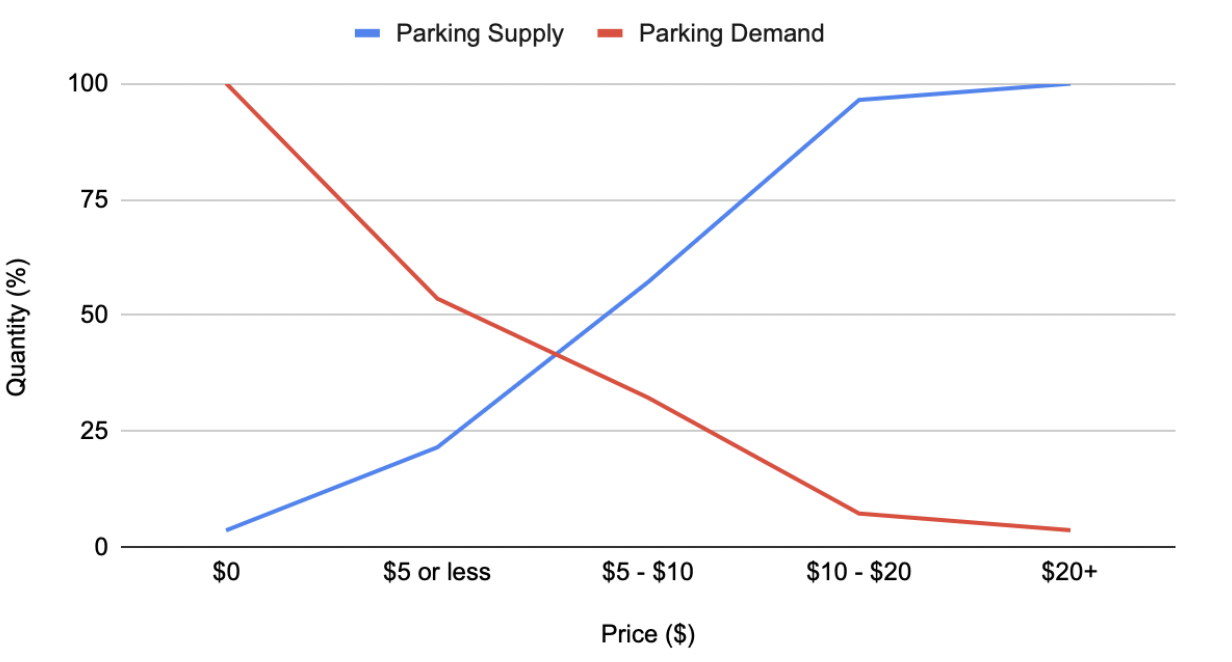
\includegraphics[width=1\textwidth]{images/cars.png}
        
        \label{fig:bird1}
    \end{figure}

\begin{figure}[ht]
        \centering
        \caption{Supply and Demand for Delivering Supers}
        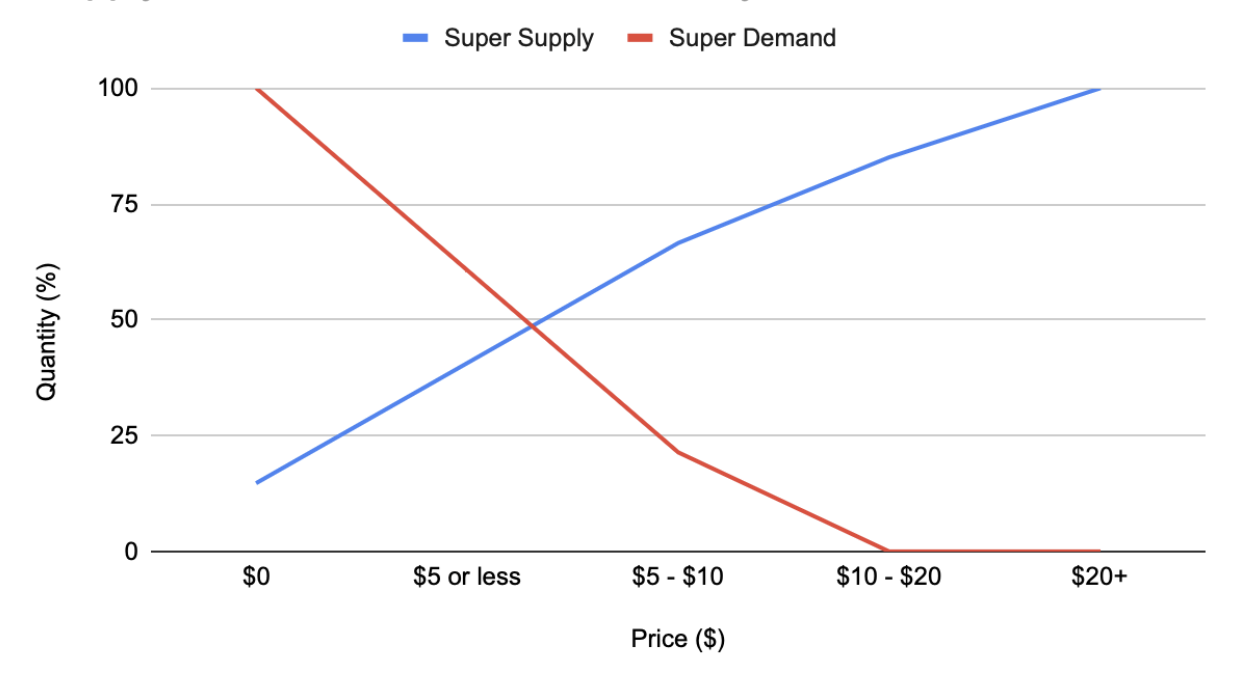
\includegraphics[width=1\textwidth]{images/supers.png}
        
        \label{fig:bird1}
    \end{figure}

\begin{figure}[ht]
        \centering
        \caption{Most Wanted Service on Campus}
        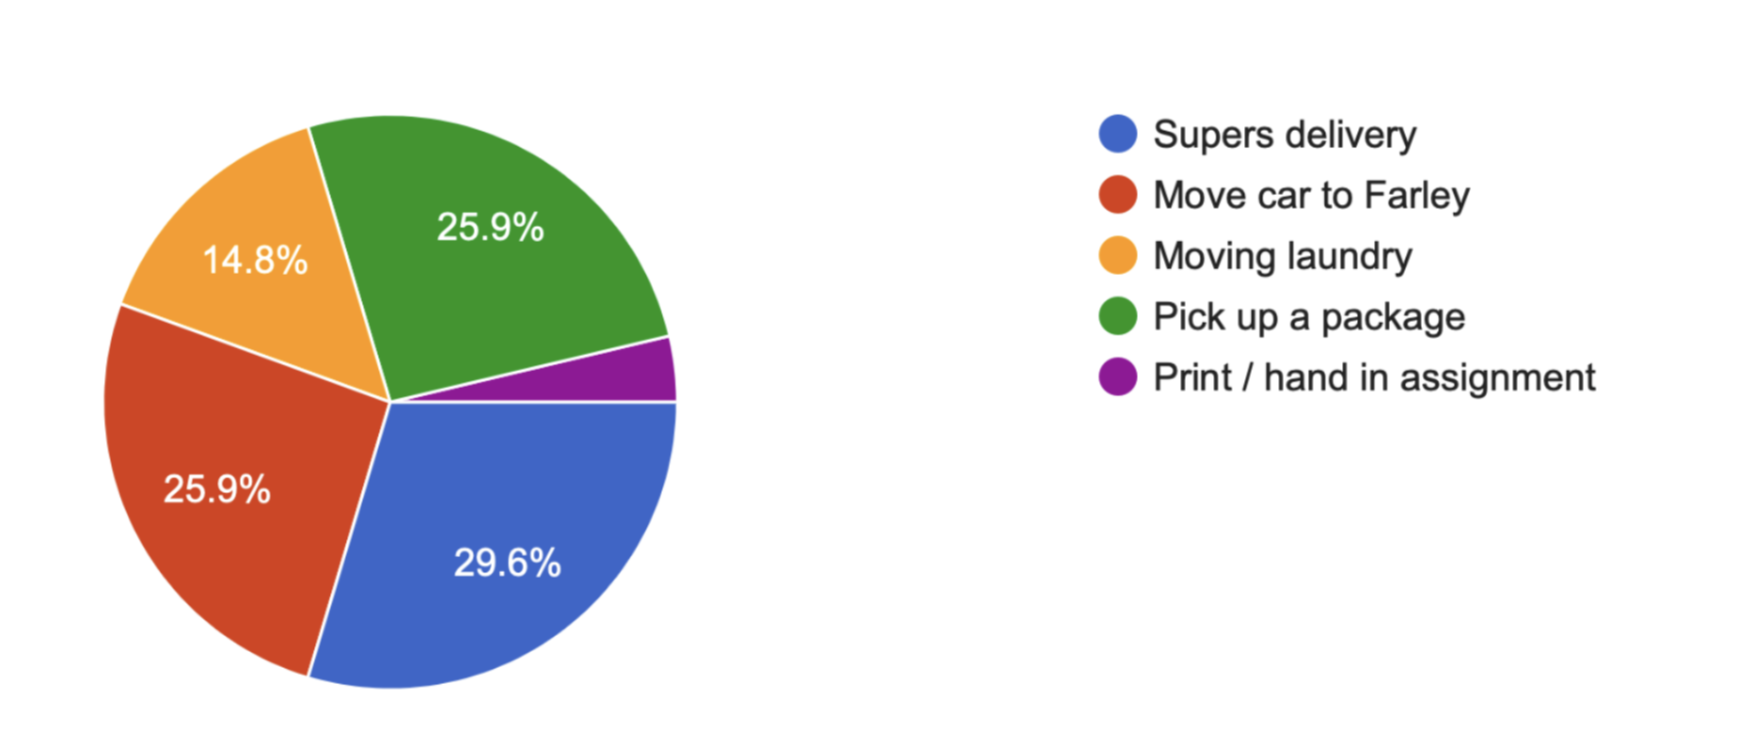
\includegraphics[width=1\textwidth]{images/pie.png}
        
        \label{fig:bird1}
    \end{figure}


\clearpage 
\section{Working Prototype Data}

After completing our initial interactive Figma prototype we had classmates test our product. We polled four students from the class and below are their major complaints and suggestions. \\


\noindent \textbf{Working Prototype (PQ4) Suggestions and Complaints:}
\begin{itemize}
\item Labels have a lack of naming clarity
\begin{itemize}
\item “My tasks” and “Active deliveries” have no continuity in what the actions are called.
\end{itemize}
\item Initial feature to “Counter” offer the poster of the task was unintuitive and many interviewees did not understand its purpose.
\item Lack of log showing your currently active tasks that youve posted, or the tasks that youve accepted to complete for others
\item Some users had difficulty navigating to the main feed after posting their task.
\item No clear way to navigate back in the application and a user was stuck in a loop while trying to navigate out of the profile page.
\end{itemize}


\section{Feedback Day Data}

After having completed a fully passable product with nearly complete functionality we had our test users register an account and post a task on Tascii and then register an account and place a Doordash order. Below are the individual's times to do so. We did this to compare time to completion and ease of use between our product and a similar competitor. Below are our results. We recorded the total time to complete the aforementioned steps and had the user select three words from a randomized list we provided. (The list had equal positive and negative terms.)

\begin{figure}[ht]
        \centering
        \caption{Supply and Demand for Moving Cars}
        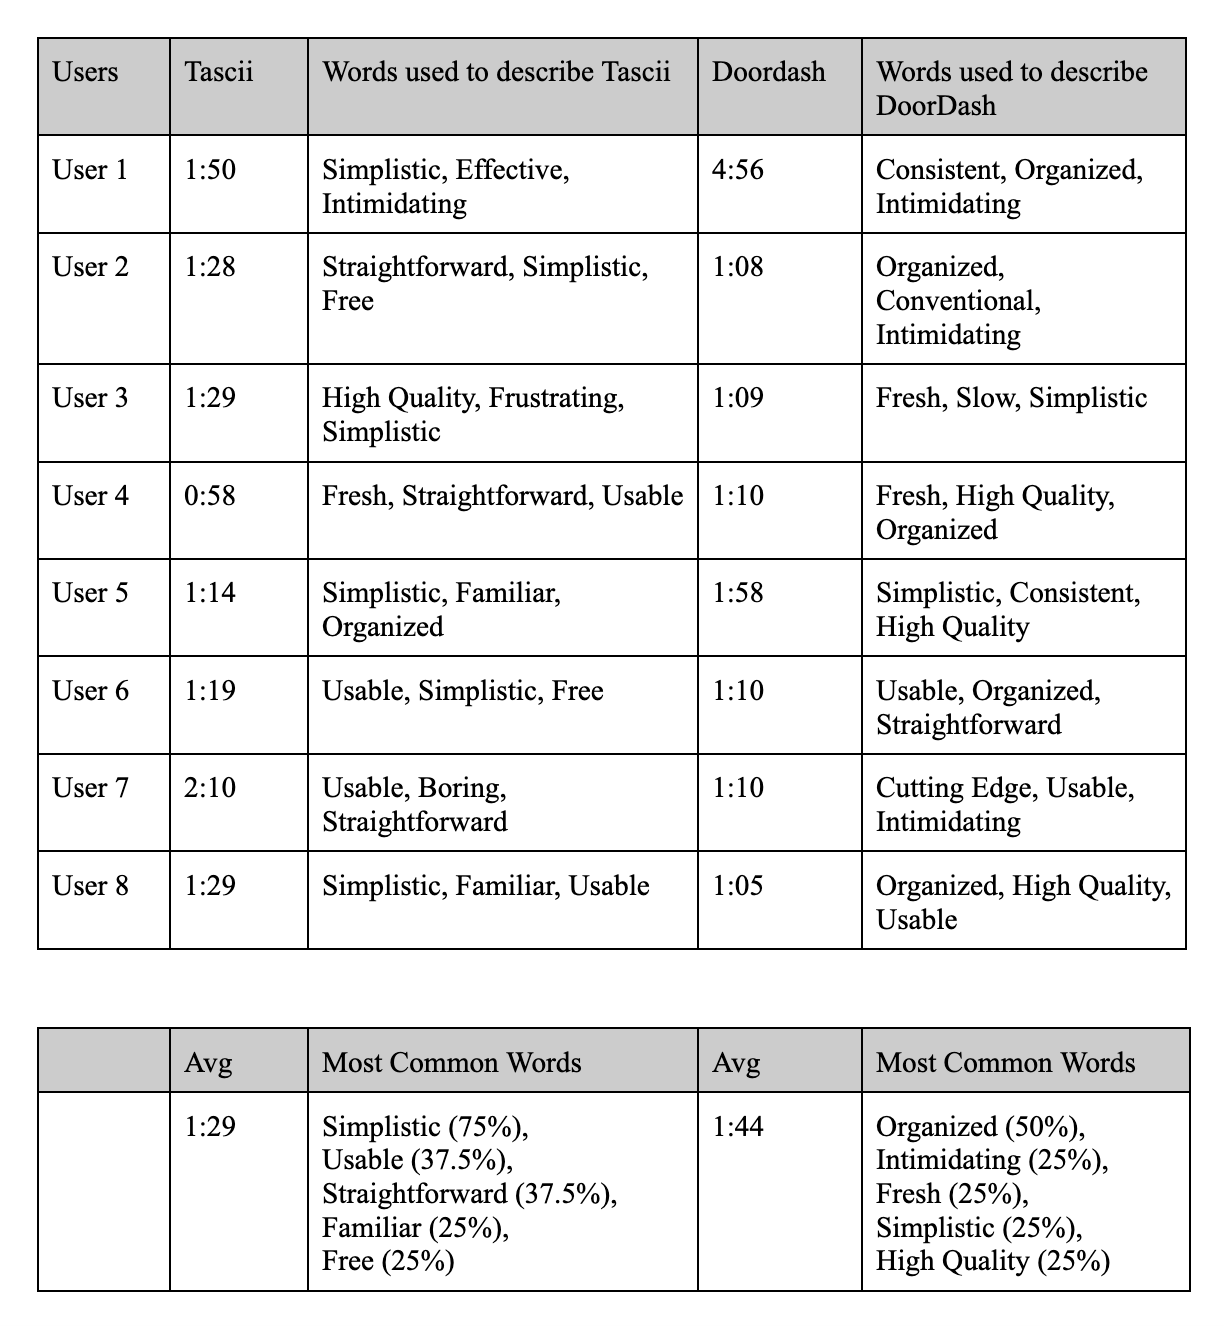
\includegraphics[width=1\textwidth]{images/Table.png}
        
        \label{fig:Data Table}
    \end{figure}
